\newcommand{\aconv}[0]{$\alpha$-conversion}
\newcommand{\bred}[0]{$\beta$-reduction}
\newcommand{\ered}[0]{$\eta$-reduction}
% CREATED BY MAGNUS GUSTAVER, 2020
\chapter{Theory}
% Kan skriva ut den här när vi har skrivit fler delar av detta kapitel
This chapter covers the theory and common problems of modern programming languages blah blah blah.

\section{Lambda calculus} \label{Lambda calculus}
% \begin{itemize}
%     \item Good references: \citep{church} \citep{church_1940} \citep{girard1986system}
%     \item Also see planning report 
% \end{itemize}

Lambda calculus is a formal mathematical logic system discovered by Alonzo Church \citep{church}. 
The system consists of three rules and three reductions:
\newline
\begin{center}
    $x$ - variable \\
    $\lambda x. M$ - abstraction \\
    $M N$ - application \\
\end{center}

In common mathematical notation abstraction can be represented by $f(x) = M$, and application by $f(N)$, where $f$ is the aforementioned function.
\newline

% Kinda ugly with enumerate but I would like a way for it to feel enumerated.
The first of the three reductions is called \aconv{}. It is the process of renaming all bound variables in a term without changing the semantics
of the term. For instance, consider the following term $\lambda x . x$, performing \aconv{} using $y$ the term would end up as $\lambda y. y$, which semantically has the same meaning. Thus the two expressions are said to be $\alpha$-equivalent.
\newline

The second is the \bred{}. The \bred is a reduction where the the bound variable in an abstraction is replaced with the argument term.
An example is the following term $(\lambda x. x) (\lambda y. y y)$. Performing one \bred{} on the term would yield ($\lambda y. y y$).
\newline

\todo[inline]{This paragraph is not entirely correct. Eta-reduction is more than this}
The third of the three reductions is the \ered{}. It is a way to express the equality between two terms, more formally this is known as the axiom of extensionality \citep{ENDERTON197717}. The following two terms are equal by \ered{}: $\lambda x . f x$ and $f$, as long as $x$ does not appear as a free variable in $f$.
\newline

\todo[inline]{Fix the flow of the text. It does not flow well here}
Lambda calculus is Turing-complete, which in essence means it is able to express anything a real-world general-purpose computer can express CITATION HERE.

\section{Simply typed lambda calculus}

Simply typed lambda calculus is an extension to lambda calculus introducing type symbols and the type constructor ($\rightarrow$)\citep{church_1940}. For instance, consider the following:
if the term $M : \alpha \rightarrow \beta$ and $N : \alpha$ are well-formed terms, then the following term $MN$ would have the type $\beta$.
\newline

Because of the extra restrictions introduced, simply typed lambda calculus is not Turing-complete \todo[inline]{CITATION HERE}.


\section{Type system}
The Curry-Howard correspondence relates the simply typed $\lambda$-calculus 
to intuitionistic logic \citep{smolka-notes}. 
The correspondence describes the construction and deconstruction of types, for instance,
the function connective $\rightarrow$ constructs a function \citep{howard-1980}.
In logic, this corresponds to introduction and elimination rules. Also, the function connective $\rightarrow$ corresponds to implication $\implies$. 
\\
\\
Type systems can be designed by combining introduction and elimination rules.
For example, abstraction $\lambda x.e$ and application $e_1 e_2$ can be type checked by the introduction and elimination rules for $\rightarrow$. 
\begin{center}
\vskip 1em
\AxiomC{$\Gamma, (x : A) \vdash e : B$}
\RightLabel{$\rightarrow$I}
\UnaryInfC{$\lambda x.e : A \rightarrow B$}
\DisplayProof
\hskip 1.5em
\AxiomC{$\Gamma \vdash e_1 : A \rightarrow B$}
\AxiomC{$\Gamma \vdash e_2 : A$}
\RightLabel{$\rightarrow$E}
\BinaryInfC{$e_1 e_2 : B$}
\DisplayProof
\vskip 1em
\end{center}
The judgments use the form $\Gamma \vdash e : A$, read "in context $\Gamma$, term e has type A". 
$\Gamma$ gives the type of the free variables in $e$, and
the notation $\Gamma , (x : A)$ is the context that extends $\Gamma$ by associating the identifier $x$ with type $A$.
Notice that the introduction rule introduces the connective
in the conclusion, while the elimination rule eliminates it from the premises. 
The type-checking algorithm can be mechanically derived from the rules. To check if the abstraction $\lambda x.e$ has type $A \rightarrow B$: extend the context with $x : A$ and check if the proposition $e : B$ holds.
Similarly, the application $e_1 e_2$ have type $B$ if $e_1$ and $e_2$ have type $A \rightarrow B$ and $A$ respectively.

\todo[inline]{Type systems are tradeoffs}
\todo[inline]{Type checking is the process of checking if a given proof holds}
\todo[inline]{Type inference is the process of creating a proof for a given proposition}





\subsection{Hindley-Milner}
\begin{itemize}
    \item The Hindley-Milner type system presents a fairly simple way system for type inference and type checking in polymorphic lambda calculus.
    \item One advantage is complete type inference, no annotations are required at all
    \item It has show faily simple to extend to user defined data types as well as case expressions.
    \item Error messages are hard to report well, as an ill-typed program is first detected in the unification part
\end{itemize}

\emph{This text assumes we have already argued for why a type system is favourable}


\subsection{Bidirectional}
\begin{itemize}
    \item popular for its scalability, error reporting, and ease of implementation \citep{bidir-gadts}.
    \item Bidirectional type checking uses two modes: type checking and type synthesis. Checking is easier and allows for a more expressive type system but it requires explicit annotations. Synthesizing a program is harder and undecidable for some language features \citep{bidir}.
    \item The combination of checking and synthesizing means that there are multiple ways to create a typing judgment. For example, there are eight different rules for a judgment with two premises and one conclusion \citep{bidir}.   
   \item Dunfield and Krishnaswami \citep{bidir} defined general design criteria for a bidirectional type system. The design criteria are:
   \begin{itemize}
       \item Mode-correctness, no guessing of types.
       \item Completeness, all terms match at least one of the rules.
       \item Size, fewer rules are easier to work with.
       \item Annotation character, sensible annotations. Annotations should be lightweight, predictable, stable, and legible.
   \end{itemize}
   \item \citep{bidir} also presented a method for creating such a typing system, which is an alteration of the Pfenning recipe \citep{pfenning-recipe}. 
   The typing rules are divided into two forms of rules: introduction and elimination rules. Introduction rules introduce a connective in the conclusion, while an elimination rule eliminates a connective present in one of the premises. A connective connects multiple formulas, for instance, abstraction $\lambda x. e$ and let expressions $let x = e in e'$.
   \item Subsumption is an extra checking rule which accepts synthesizable expressions such as application $e_1 e_2$ \citep{bidir}. This is possible due to checking containing more information than synthesizing. Changing in the other direction is thus not possible. 
   
   
\end{itemize}


\section{LLVM}
very rough :))

A part of creating a programming language is making a representation of runnable by computers,
for this task, some sort of assembly language is a suitable solution.
\\

An assembly language is a low-level programming language that closely represents a machine's actual 
CPU instructions. These languages are often quite simple, consisting of CPU instructions known as opcodes,
labels to allow for branching code, and in some cases, features like macros.
\todo[inline]{insert example assembly code?}
\\

There are a variety of available assembly languages, including the x86 family, the ARM assembly languages, and more.
However, these flavors of assembly come with a big flaw, which is being platform dependant, and in some cases 
CPU model dependant. For example; a program written in ARMv7 assembly will not run on an x86 CPU, and the same goes
for x86 assembly, which can not run on an ARMv7 CPU.
\\

The creation of LLVM started in 2000, and while it was initially developed to explore dynamic compilation techniques, 
it has over time evolved to be quite a large compiler framework encompassing many different smaller projects.
One of these projects is the high-level intermediate representation assembly language LLVM IR, which is a 
high-level assembly language that can be compiled into many different assembly languages, 
such as the x86 family or the ARM languages mentioned before.

This intermediate language closely resembles the lower-level assembly languages, while also shaking things up
by having a type system(a rarity among assembly languages), type declarations, function definitions, and more.
\\

LLVM IR is written in single static assignment form (SSA), which just adds the rule that variables may only 
be assigned once. This guarantee makes optimization of the IR code easier, as unused and unnecessary variables
can easily be optimized away and quite a few other optimization algorithms make use of it,
although it comes at the cost of being harder to translate to compared to other assembly languages, depending on
the source language.
\todo[inline]{insert sources}
\todo[inline]{insert example}

% Behöver verkligen inte vara den första sectionen utav kapitlet
% Jag antar här att teori ska va presens som introduktion
\section{Memory management}
Memory is a fundamental and finite resource that allows computers to store data which leads to the possibility
of executing programs that have to be loaded into memory. Programs need memory to store data such as variables
and objects in memory during execution. Due to memory being a finite resource, its amount limits the size and
the capabilities of an executing program. Since a computer's memory is shared across multiple programs
executing concurrently, one single program mustn't try to allocate or use all of the
available memory, resulting in limitations on the rest of the system and executing programs. Therefore
it is important to minimize the amount of memory allocated to or by a program, without
interfering with its execution.\\

In modern high-level programming languages such as Java and Haskell, memory is automatically managed by
their runtimes (code that is executed during the program's execution which enables the program to interact
with system resources). Depending on the use case of the language, the runtime varies in size. For example, lower-level
languages such as C have very small runtimes since the language is already close to using system resources like
memory, close meaning that a developer in this language can directly request resources from the system
without the use of the language runtime. In high-level languages system resources are allocated by
the runtime, where the runtime can efficiently keep track of used and unused but allocated memory.
Algorithms for freeing up memory can then be applied by the runtime on this data to minimize the amount
of memory used by the program. This process of freeing up memory is also well-known as garbage collection.\\

\subsection{Memory layout and program interaction}

For a program to be executed it has to be compiled and then loaded into memory by the operating system.
The compiled program is split into smaller segments called stack, heap, text, bss, and data [insert source].
The stack segment contains the call stack of the program, which is used for function calls, saving registers,
and storing local variables. The bss and data segments are less important and are used for storing
global variables in the program, uninitialized and initialized respectively. The text segment
contains the program code in byte-code format used by the central processing unit (CPU) to execute the
compiled program. The most important segment for memory management is the heap segment, which is where allocated
objects live in system memory. This segment (as well as the stack segment) can grow as needed via system
calls to the operating system. Although it can grow, the stack and heap segments grow towards each other
as indicated by the arrows in figure [X, insert figure], so each program has a finite but varying amount of memory.\\ % [double check statement above]

A program can request heap memory either explicitly by the developer in lower-level languages, or by
a runtime in higher-level languages upon object creation. Where these objects live on the heap, and
what addresses their memory space starts depends on implementation details by the operating system.
In Linux operating systems and C, memory can explicitly be requested by calling the function
malloc, which tries to allocate memory on the heap. This function uses the internal system-call sbrk
to request more resources from the operating system to extend the heap size to allow
more memory for a program \citep[p.~188]{KandR}. Although sbrk allows the heap to grow, the amount it
can grow before it hits the stack is limited as previously mentioned. This problem introduces
the solution of using another system call, called mmap, which allocates and maps larger chunks of memory
requested. The system-call mmap is used in the current implementation of malloc in the GNU C library \citep{mallocSrcCode}.
Since malloc uses these two different allocation strategies, objects may be scattered across memory
depending on their size and the flow of the executing program. This makes the process of freeing
up unused memory tricky since it is impossible to know which objects are still in use just by
looking at the memory, compared to the stack where it is easy to distinguish stack frames and determine
the lifespans of variables.

\subsection{Mark and sweep algorithm}
The mark and sweep algorithm is one of the earliest forms of automatic memory management, invented
in the early 60s \citep{MandSproject}. This algorithm is known as a "stop-the-world" algorithm,
which means that the execution of the program is paused while the collector (the implementation
of the algorithm) analyses the heap and program memory, and is later resumed when the collector
is finished. The collector is triggered when an allocation is requested but
there is not enough memory available on the heap to satisfy the request \citep[p.~18]{gcollHandbook}.
The program is then
stopped briefly while the collector tries to free up memory. The process of freeing up memory is
split into two phases, the marking of alive objects and the sweeping of dead objects. Objects in
memory are considered to be alive if they can be reached directly from the current state of
memory by the program or through other objects that are already considered to be alive.
Since the heap contains all the objects ever created by the executing program, the dead objects
are merely a subset of the heap and can be easily swept by the sweep phase, where the memory
that the dead objects occupy is freed. Because of this, the complexity of the sweep phase
is fairly simple and the implementation details may not vary to a large extent.\\

The marking of objects is implementation independent since each compiler and optional runtimes
are different. The ultimate problem is where the marking phase should start (also called
the roots) and how to determine it. In the specification of the mark and sweep algorithm, it is
only implied that these roots exist and there is no description of how to acquire these root
objects or how to determine if one single object is a root object \citep[p.~19]{gcollHandbook}.
Some compiler frameworks offer tools to ease this process such as stack maps in
LLVM \citep{llvmStackMaps}. But in compilers where these kinds of tools are unavailable,
this problem is open to interpretation by the developer.



% In the following sections, examples of a figure, an equation, a table, a chemical structure, a list, a listing and a to-do note are shown.

% \section{Figure}
% \begin{figure}[H]
% \centering
% 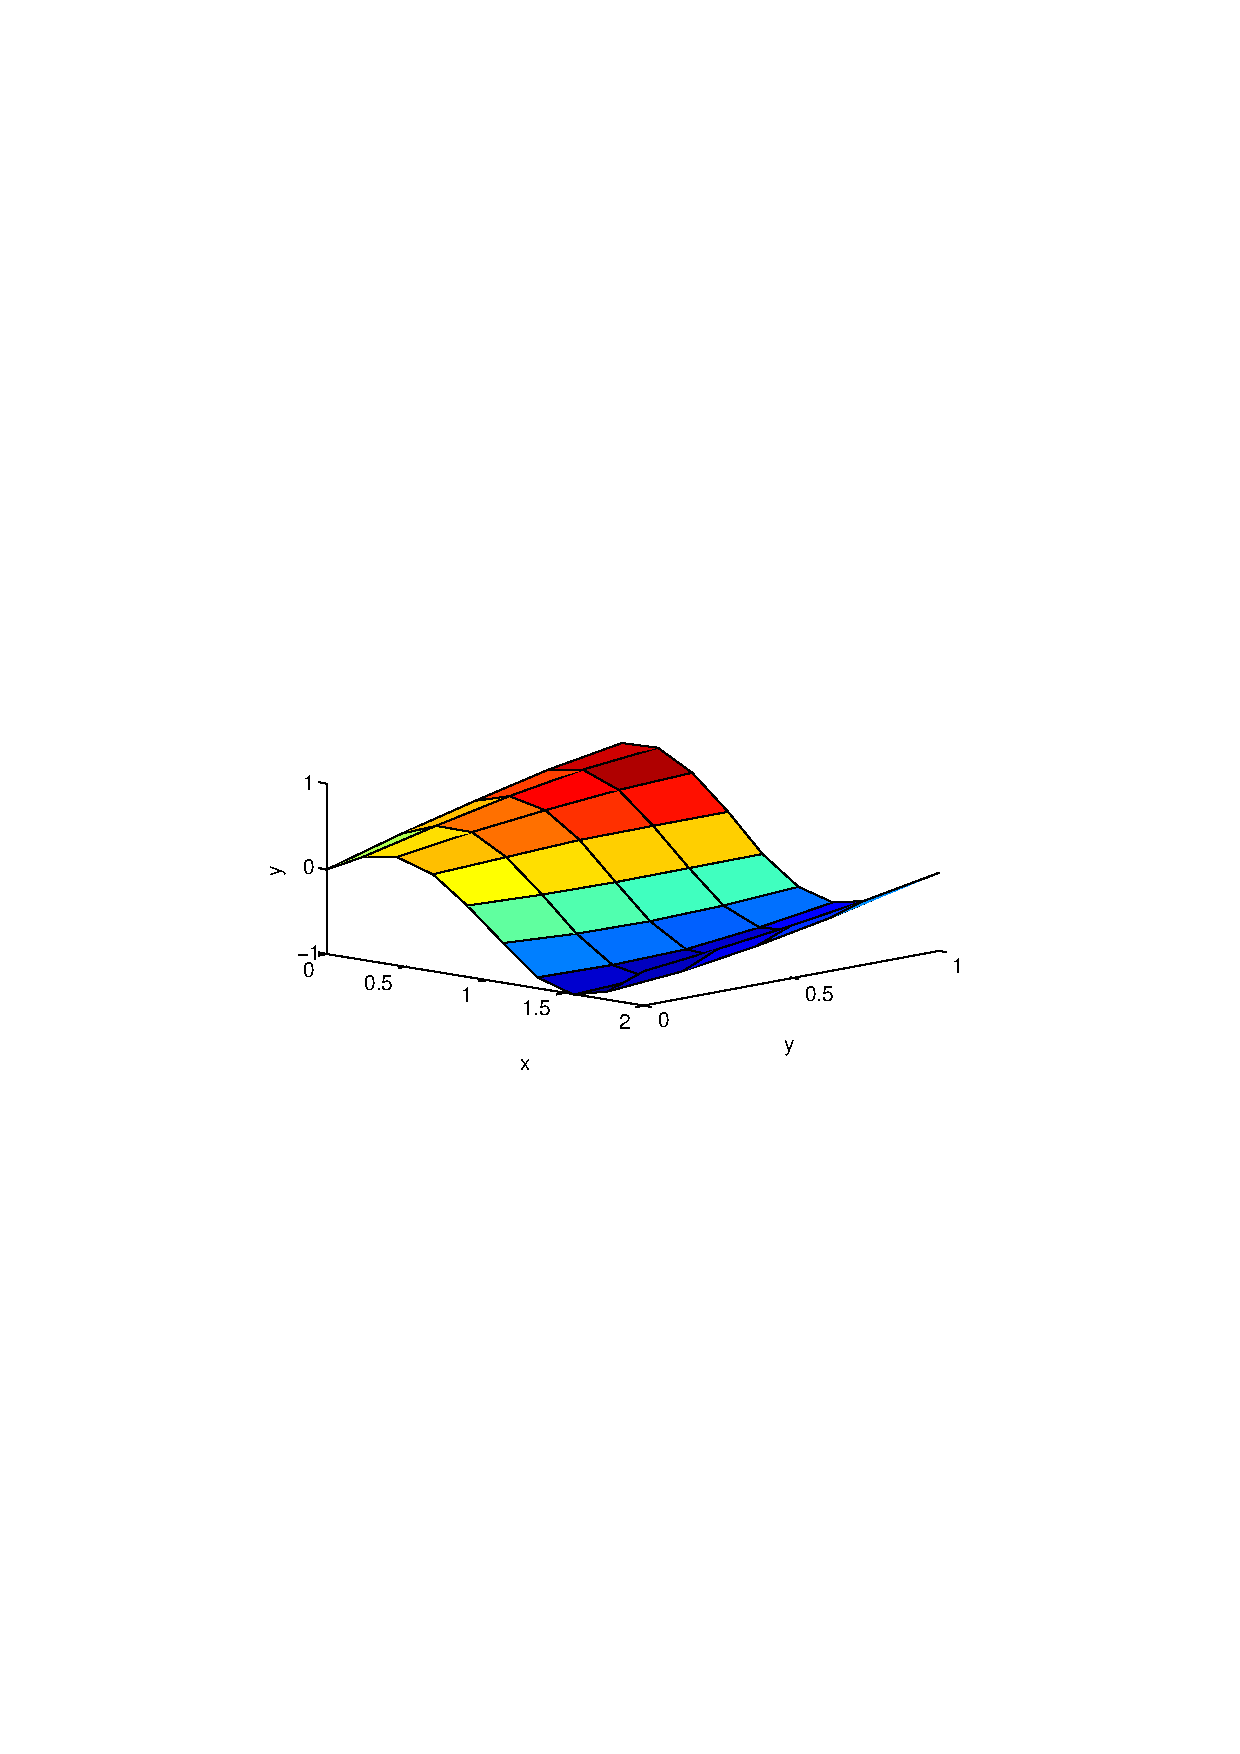
\includegraphics[width=0.45\linewidth, trim=3cm 11cm 3cm 11cm]{figure/X.pdf}
% 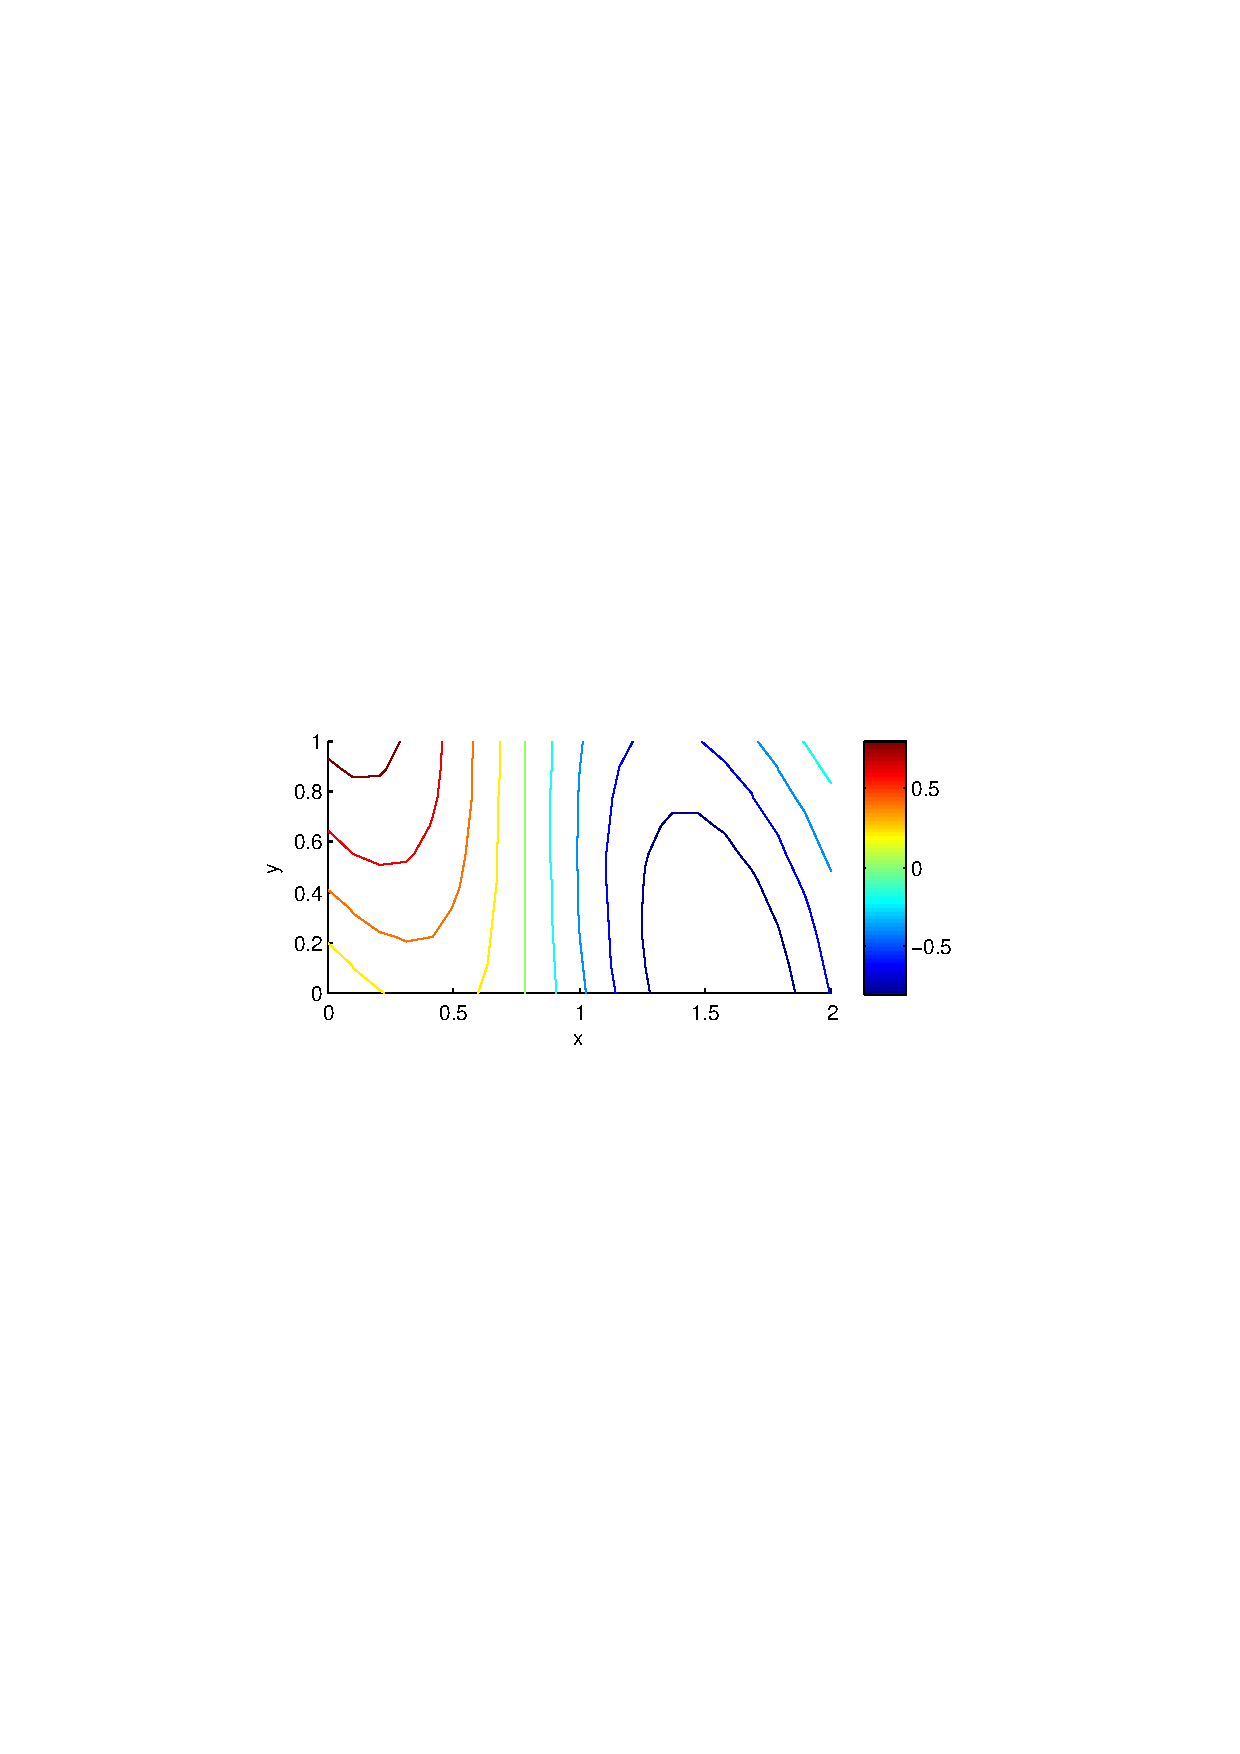
\includegraphics[width=0.45\linewidth, trim=3cm 11cm 3cm 11cm]{figure/Y.pdf}
% \caption{Surface and contour plots showing the two dimensional function $z(x,y)=\sin(x+y)\cos(2x)$.}
% \end{figure}

% \section{Equation}
% \begin{equation}
% f(t)=\left\{ \begin{array}{ll}
% 1,~~~~ & t< 1 \\
% t^2 & t\geq 1
% \end{array}\right.
% \end{equation}

% \section{Table}
% \begin{table}[H]
% \centering
% \caption{Values of $f(t)$ for $t=0,1,\dots 5$.}
% \begin{tabular}{l|llllll} \hline\hline
% $t$ & 0 & 1 & 2 & 3 & 4 & 5 \\ \hline
% $f(t)$ & 1 & 1 & 4 & 9 & 16 & 25 \\ \hline\hline
% \end{tabular}
% \end{table}

% \section{Chemical structure}
% \begin{center}
% \chemfig{X*5(-E-T-A-L-)}
% \end{center}

% \section{List}
% \begin{enumerate}
%   \item The first item
%   \begin{enumerate}
%     \item Nested item 1
%     \item Nested item 2
%   \end{enumerate}
%   \item The second item
%   \item The third item 
%   \item \dots
% \end{enumerate}

% \section{Source code listing}
% %\lstset{language=Matlab}
% \begin{lstlisting}[frame=single]
% % Generate x- and y-nodes
% x=linspace(0,1); y=linspace(0,1);

% % Calculate z=f(x,y)
% for i=1:length(x)
%  for j=1:length(y)
%   z(i,j)=x(i)+2*y(j);
%  end
% end
% \end{lstlisting}

% \section{To-do note}
% The \texttt{todo} package enables to-do notes to be added in the page margin. This can be a very convenient way of making notes in the document during the process of writing. All notes can be hidden by using the option \emph{disable} when loading the package in the settings. \todo{Example of a to-do note.}

